\documentclass[a4paper]{report}
\usepackage[ngerman]{babel}
\usepackage{tcolorbox}
\usepackage{amssymb}
\usepackage{amsmath}
\usepackage{enumitem}
\usepackage{fancyvrb}
\usepackage{sectsty}
\usepackage{siunitx}
\usepackage{bm}
\usepackage{graphicx}

\allsectionsfont{\normalfont\bfseries\itshape}


\begin{document}
\begin{titlepage}
    \centering
	{\LARGE \textsc{Spezielle Relativitätstheorie}\par}
	\vspace{1.5cm}
	{\huge\bfseries Physik\par}
	\vspace{2cm}
	{\Large\itshape Laura Thiel\par}
	{\large \today\par}
\end{titlepage}
\tableofcontents
\chapter{Einstieg SRT}
\section{Das Jahr 1905}
Im Jahr 1905 erlebte die Welt der Wissenschaft das faszinierende \textbf{"Wunderjahr"} von Albert Einstein, in dem er mit einer beeindruckenden Vielfalt an bahnbrechenden Arbeiten die Grundlagen für das Verständnis des Universums legte. Seine Veröffentlichungen in diesem Jahr sind wie ein kreativer Kosmos, der die Grenzen des Denkens erweiterte.
Einstein präsentierte nicht nur die \textbf{spezielle Relativitätstheorie}, die unsere Konzeption von Raum und Zeit revolutionierte, sondern wagte sich auch an die Hypothese der \textbf{Lichtquanten}, die die Wellen-Teilchen-Dualität des Lichts in den Fokus rückte. Sein Genie zeigte sich ebenfalls in Arbeiten zur \textbf{Brownschen Molekularbewegung} und der \textbf{Erklärung des photoelektrischen Effekts}, die die Quantenmechanik vorantrieben.
Diese wegweisenden Veröffentlichungen katapultierten Einstein in den wissenschaftlichen Olymp und ebneten den Weg für eine glanzvolle Karriere. Seine Doktorarbeit wurde 1905 in Zürich angenommen, und im darauf folgenden Jahr erhielt er den Titel "Dr. Albert Einstein". Die kontinuierliche Anerkennung führte zu seiner Beförderung in seinem Berufsfeld und kulminierte schließlich 1909 in einer Professur für Physik in Zürich.
Das Jahr 1905 markiert nicht nur den Höhepunkt von Einsteins kreativem Schaffen, sondern auch den Beginn eines erstaunlichen wissenschaftlichen Erbes, das die Welt bis heute prägt. Einsteins \textbf{Wunderjahr} bleibt eine inspirierende Quelle für alle, die die Mysterien des Universums erforschen und die Grenzen des menschlichen Denkens erweitern wollen.
\section{Einsteins Gedankenwelt}
Einsteins Gedankenwelt offenbarte sich in seiner Speziellen Relativitätstheorie, die im Volksmund gerne als \emph{"Alles ist relativ"} zusammengefasst wird. Doch der wahre Durchbruch Einsteins bestand darin, eine absolute Größe festzusetzen und so die Grundlagen der Physik zu revolutionieren.
\subsection{(Klein-)Einstein rennt dem Licht hinterher}
Einstein beschäftigte sich bereits in seiner Jugend mit Gedankenexperimenten, darunter die Vorstellung, einem Lichtstrahl hinterherzulaufen. Diese Experimente führten ihn zu bedeutenden Erkenntnissen über die Natur der Zeit und des Raums.
\subsection{Michelson und Morley Experiment}
Das berühmte Michelson-Morley-Experiment markierte einen Meilenstein in der Geschichte der Physik. Die Forscher maßen die Lichtgeschwindigkeit parallel und antiparallel zur Bahngeschwindigkeit der Erde. Ein zentrales Gedankenexperiment Einsteins während dieser Zeit war die Frage, ob er sich selbst sehen könnte, wenn er das Licht einholen würde, und was er überhaupt sehen könnte, wenn er schneller als das Licht wäre.
\subsection{Verbesserung der Messapparaturen}
In der Ära von Michelson und Morley wurden stetig verbesserte Messapparaturen entwickelt, um die Lichtgeschwindigkeit zu präzisieren. Durch den geschickten Einsatz der Erdbahngeschwindigkeit um die Sonne als Maßstab erwartete man Veränderungen in der Lichtgeschwindigkeit – ähnlich wie bei einem Boot, das konstant flussaufwärts und flussabwärts angetrieben wird.
\subsection{Ergebnis des Michelson-Morley Experiments}
\sloppy
Überraschenderweise ergab das Experiment jedoch keine Änderung in der Lichtgeschwindigkeit.
Die Physiker kamen zu dem Ergebnis, dass die Lichtgeschwindigkeit einen konstanten Wert hat: 
$$c = \SI{299792458}{\meter\per\second} \approx \SI{300000}{\kilo\meter\per\second}$$
Dies bedeutet, dass ein Einstein, der gleichförmig rennt, den gleichen Wert für die Lichtgeschwindigkeit misst wie ein ruhender Einstein. 
In diesem Kontext ist also nichts relativ; die Lichtgeschwindigkeit ist schlichtweg eine absolute Größe.
\chapter{Einstein'sche Postulate und Bezugssysteme}
\begin{tcolorbox}
	\textbf{Postulieren:} Eine unbedingte Forderung oder vorläufig akzeptierte These, abgeleitet vom lateinischen "postulāre" ('verlangen, begehren, fordern'). Es bezeichnet eine vorläufig angenommene Aussage, die möglicherweise noch nicht bewiesen ist.
\end{tcolorbox}\
\begin{flushleft}
	Einstein legte lediglich zwei grundlegende Annahmen oder Postulate fest, um seine wegweisende Theorie der Speziellen Relativitätstheorie zu entwickeln. Bereits kennengelernt haben wir die Konstanz der Lichtgeschwindigkeit (c), die experimentell nie widerlegt wurde und ein fundamentaler Bestandteil der Theorie ist. 
	Im nächsten Abschnitt werden wir uns mit dem zweiten Postulat beschäftigen, dem sogenannten Relativitätsprinzip.	
\end{flushleft}
\section{Bezugssysteme und Inertialsysteme}
Das mechanische \textbf{Relativitätsprinzip} geht schon auf \textbf{Galilei} und \textbf{Newton} zurück. In den folgenden Unterkapiteln geht es nun um das 'Relative' in der Speziellen Relativitätstheorie (ab hier SRT genannt).
\subsection{Situation 1}
Einstein und Newton bewegen sich in ihren Zügen mit jeweils einer Geschwindigkeit von \(v_{\text{Newton}} = v_{\text{Einstein}} = 47 \, \text{km/h}\). Dadurch bewegen sich die beiden relativ zueinander mit einer Geschwindigkeit von \(v_{\text{relativ}} = 0 \, \text{km/h}\).
Angenommen, Newton führt auf seinem gleichförmig bewegten Zug einen Versuch durch, beispielsweise das Fallenlassen eines Apfels, so würde Einstein dies genauso wahrnehmen wie Newton. Diese Situation wäre gleich, selbst wenn beide Wissenschaftler in einem Labor stehen würden.
\subsection{Situation 2}
Im zweiten Szenario würde Einstein in seinem Zug eine Relativgeschwindigkeit von \(v_{\text{relativ}} = 65 \, \text{km/h} - 47 \, \text{km/h} = 18 \, \text{km/h}\) in Bezug auf Newton messen. Wenn Einstein nun einen Apfel fallen lässt, würde dieser aus seiner Perspektive senkrecht nach unten fallen, während Newton eine Wurfparabel sehen würde, da sich der Apfel aus seiner Perspektive zusätzlich mit \(v_{\text{relativ}}\) nach vorne bewegt.
Wenn dieser Versuch von Einstein in einem ruhenden Labor durchgeführt wird, müsste Newton mit \(v_{\text{relativ}} = 18 \, \text{km/h}\) daran vorbeijoggen, um dieselbe Beobachtung zu machen.
\subsection{Relativitätsprinzip}
Das führt uns zum zweiten Postulat, dem Relativitätsprinzip. In unbeschleunigten Bezugssystemen sollen alle physikalischen Gesetze gleich sein. Galileo Galilei erkannte dies bereits 1638 im Inneren eines ruhigen Schiffes.
In beschleunigten Bezugssystemen variieren die Gesetze aufgrund von Scheinkräften, wie beim Anfahren eines Autos. Im Gegensatz dazu fallen Objekte in unbeschleunigten Bezugssystemen, wie einem gleichförmig fahrenden Zug, senkrecht nach unten. Solche Systeme werden als Inertialsysteme bezeichnet, in denen die physikalischen Gesetze einheitlich gelten, ohne einen absoluten Ruhepunkt.
\section{Lichtuhr}
Die Einstein'schen Postulate sind eigentlich einfach und schon ausreichend für das elementare Gedankenexperiment: die Lichtuhr.
Diese besteht aus einem Inertialsystem, welches durch zwei Spiegel begrenzt ist und einem Photon, das sich periodisch zwischen den beiden Spiegeln mit der konstanten Lichtgeschwindigkeit \(c\) bewegt.
\begin{flushleft}
\begin{tcolorbox}
	Die Lichtuhr tickt in jedem Inertialsystem \textbf{gleich schnell}, da die Lichtgeschwindigkeit \(c\) \textbf{invariant} ist.
\end{tcolorbox}
\end{flushleft}
\section{Einstein'sche Postulate}
\begin{flushleft}
	\begin{tcolorbox}
		\textbf{1. Postulat - Relativitätsprinzip:}
		\newline
		Bezugssysteme, die sich relativ zueinander mit konstanter Geschwindigkeit bewegen, nennt man \textbf{Inertialsysteme}. Alle Inertialsysteme sind \textbf{gleichberechtigt}, und physikalische Vorgänge laufen in ihnen \textbf{identisch} ab.
		\newline
		\newline
		\textbf{2. Postulat - Konstanz der Lichtgeschwindigkeit:}
		\newline
		In allen Inertialsystemen beträgt die Vakuumlichtgeschwindigkeit \(\mathbf{c = 299,792 \, \text{km/s}}\), unabhängig von der Momentangeschwindigkeit der Lichtquelle.
	\end{tcolorbox}
\end{flushleft}
\chapter{Relativität der Gleichzeitigkeit}
In der klassischen Welt, bei Geschwindigkeiten weit unterhalb der \textbf{Lichtgeschwindigkeit}, synchronisiert man Uhren, indem man ihre Taktfrequenzen vergleicht. Bei Bauern auf dem Feld war dies schwieriger, da das Zwölfuhrläuten im Vergleich zu Dorfbewohnern zeitversetzt wahrgenommen wurde.
Die Herausforderung bestand darin, zwei fest installierte Kirchturmuhren trotz der \textbf{Schallgeschwindigkeit} von \( \underline{330 \, \text{m/s}} \) zu synchronisieren.
\begin{tcolorbox}
	Aufgrund der Konstanz der \textbf{Lichtgeschwindigkeit} \(c\) können Informationen nicht schneller als mit Lichtgeschwindigkeit übertragen werden. Um zwei Uhren zu synchronisieren, müssen sie gleichzeitig ticken.
	\newline
	\newline
	Zwei Uhren an verschiedenen Orten innerhalb eines gemeinsamen \textbf{Inertialsystems} werden durch ein \textbf{Lichtsignal} synchronisiert, das vom Mittelpunkt ihres Abstands ausgeht.
	\newline
	Wenn zwei Uhren in einem gemeinsamen \textbf{Inertialsystem} synchronisiert sind, gilt dies nicht für alle anderen \textbf{Inertialsysteme}.
	\newline
	Diese Erkenntnis lässt sich auch auf \textbf{Ereignisse} anwenden: Wenn zwei \textbf{Ereignisse} innerhalb eines \textbf{Inertialsystems} gleichzeitig stattfinden, geschieht dies nicht in allen anderen \textbf{Inertialsystemen}.\end{tcolorbox}
\chapter{Zeitdilatation}
\begin{tcolorbox}
	Die \textbf{Zeitdilatation}, basierend auf dem lateinischen Wort "dilatare" für 'dehnen' oder 'aufschieben', ist ein Effekt der \textbf{Relativitätstheorie}. Sie bewirkt, dass interne Prozesse eines physikalischen Systems langsamer erscheinen, wenn sich das System relativ zum Beobachter bewegt.
\end{tcolorbox}
\textbf{"Bewegte Uhren verlangsamen ihre Zeitmessung."}
\section{Herleitung des Lorentzfaktors $\gamma$}
Der Lorentz-Faktor, durch \( \gamma \) dargestellt, leitet sich von den Lorentz-Transformationen in der speziellen Relativitätstheorie ab. Der Lorentz-Faktor ist definiert als:

\[ \gamma = \frac{1}{\sqrt{1 - \frac{v^2}{c^2}}} \]

\begin{flushleft}
	Ausdruck für \( \gamma \) ableiten:
\end{flushleft}

\begin{align*}
t' &= \gamma t - \frac{\gamma vx}{c^2} \\
x' &= \gamma x - \gamma vt
\end{align*}

\begin{flushleft}
	Um \( t \) und \( x \) zu entfernen, quadrieren wir beide Gleichungen und addieren sie:
\end{flushleft}

\begin{align*}
t'^2 - x'^2 &= \gamma^2 t^2 - \frac{2\gamma vx}{c^2} t + \frac{\gamma^2 v^2 x^2}{c^2} - \gamma^2 x^2 + 2\gamma vt - \gamma^2 v^2 t^2
\end{align*}

\begin{flushleft}
	Ordnen und Gruppieren gleicher Terme:
\end{flushleft}

\begin{align*}
t'^2 - x'^2 &= (\gamma^2 - \gamma^2 v^2) t^2 - (\gamma^2 - \gamma^2 v^2) x^2 + (\frac{2\gamma}{c^2} - 2\gamma vt) x \\
&= \gamma^2 (1 - v^2) t^2 - \gamma^2 (1 - v^2) x^2 + \frac{2\gamma}{c^2} x
\end{align*}

\begin{flushleft}
	Mit \( 1 - \frac{v^2}{c^2} = \frac{1}{\gamma^2} \) vereinfachen:
\end{flushleft}

\begin{align*}
t'^2 - x'^2 &= \gamma^2 (c^2 - v^2) t^2 - \gamma^2 (c^2 - v^2) x^2 + \frac{2\gamma}{c^2} x \\
&= \gamma^2 c^2 (t^2 - x^2) + \frac{2\gamma}{c^2} x
\end{align*}

\begin{flushleft}
	Ordnen und \( c^2 \) herausfaktorisieren:
\end{flushleft}

\begin{align*}
c^2 (t'^2 - x'^2) &= \gamma^2 c^4 (t^2 - x^2) + 2\gamma x \\
c^2 (t'^2 - x'^2) &= c^2 (t^2 - x^2) + 2\gamma x
\end{align*}

\begin{flushleft}
	Durch \( c^2 \) teilen:
\end{flushleft}

\begin{align*}
t'^2 - x'^2 &= t^2 - x^2 + \frac{2\gamma}{c^2} x
\end{align*}

\begin{flushleft}
	Nach \( \gamma \) auflösen:
\end{flushleft}

\begin{align*}
\frac{2\gamma}{c^2} x &= t'^2 - x'^2 - t^2 + x^2 \\
\frac{2\gamma}{c^2} x &= -(\Delta t)^2 + (\Delta x)^2 \\
\gamma &= \frac{1}{\sqrt{1 - \frac{v^2}{c^2}}}
\end{align*}

\begin{flushleft}
	Daher ist der Lorentz-Faktor (\( \gamma \)) abgeleitet.
\end{flushleft}
\section{Der Lorentzfaktor - eine Beispielrechnung}

Die Beziehung lautet \( t = \frac{t_0}{\sqrt{1 - \left(\frac{v}{c}\right)^2}} \), wobei der Faktor \( \frac{1}{\sqrt{1 - \left(\frac{v}{c}\right)^2}} \) oft als \( \gamma \) abgekürzt wird und als Lorentzfaktor bekannt ist.
Der Lorentzfaktor ist ein Maß für die relativistische Zeitdilatation. Ein Lorentzfaktor von \( \gamma = 2 \) würde bedeuten, dass aus Sicht von Albert Einstein die bewegte Uhr nur halb so schnell tickt wie seine eigene Uhr.
Angenommen, man würde auf einem Zug in seinem Bezugssystem ein \( t_0 = 5 \) Minuten dauerndes Ereignis, wie das Kochen eines Eies, beobachten. Dann würde Einstein aus seinem System heraus für diesen im Zug ablaufenden Vorgang \( t = \gamma \cdot t_0 = 2 \cdot 5 \) Minuten messen, also \( t = 10 \) Minuten.
In der Relativitätstheorie gibt man Geschwindigkeiten oft relativ zur Lichtgeschwindigkeit an. Für \( v = 0,8c \) ergibt sich beispielsweise der Lorentzfaktor \( \gamma \) zu:
\[ \gamma = \frac{1}{\sqrt{1 - \left(\frac{0,8c}{c}\right)^2}} = \frac{1}{\sqrt{1 - 0,64}} \]
Weiter vereinfachen wir:
\[ \gamma = \frac{1}{\sqrt{0,36}} = \frac{1}{0,6} \]
Daher beträgt der Lorentzfaktor in diesem Fall etwa \( \gamma \approx 1,67 \).
\section{Übung zur Zeitdilatation}
\subsection{Aufgabenstellung}
\begin{figure}[h]
	\centering
	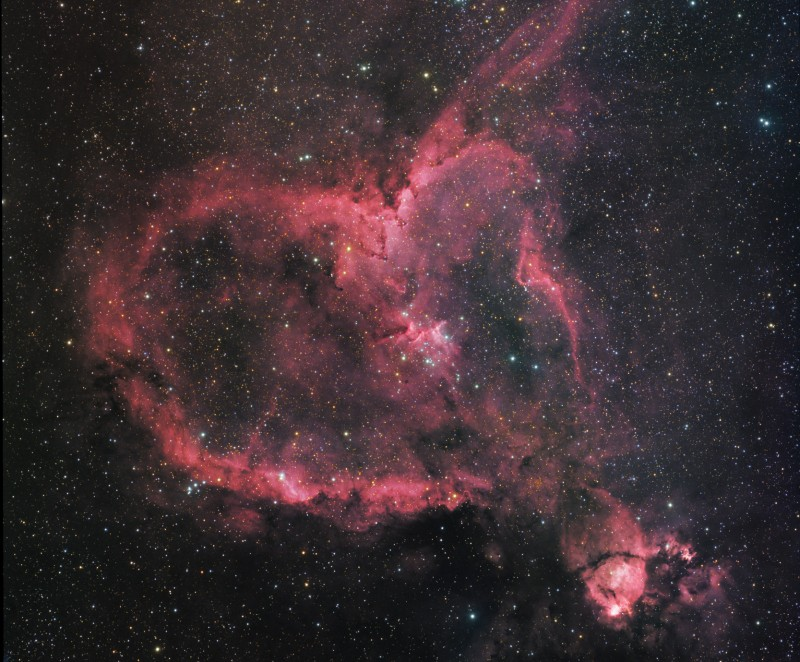
\includegraphics[scale=.5]{images/Heart_Nebula.jpeg}
	\end{figure}
\begin{flushleft}
	Julia hat sich unsterblich in Sir Isaac Newton verliebt. Gemeinsam wollen sie der tristen Insel Albion entkommen und ihre "rosa Phase" aus Sicht eines Erdbewohners auf das Doppelte verlängern. Als Ziel wählen Sie - wie romantisch - den \(7500 \, \text{Lj}\) entfernten Herznebel.
\begin{enumerate}
    \item Geben Sie den für die Verdopplung der Zeit aus Erdsicht notwendigen Wert des Lorentzfaktors an.
    \item Berechnen Sie mit dem Ergebnis aus Teilaufgabe 1 die Geschwindigkeit \(v\) des Raumschiffs Rocket des Liebespaars.
    \item Sir Isaac Newton lässt abends die 20-minütige Fantasie-Ouvertüre "Romeo und Julia" von Tschaikowsky erklingen. Berechnen Sie die Zeit, die ein Erdbeobachter für das Abspielen dieser Ouvertüre messen würde.
    \item Berechnen Sie aus der Sicht eines Erdbeobachters die Reisedauer der beiden Liebenden bis zum Herznebel.
\end{enumerate}
\end{flushleft}
\subsection{Lösung}
\begin{figure}[h]
	\centering
	\includegraphics[scale=.7]{images/Lösung_Zeitdilatation.png}
	\end{figure}
\section{Zusammenfassung}
\begin{tcolorbox}
	Im Kontext der Speziellen Relativitätstheorie gilt der Zusammenhang
\[ \Delta t = \gamma \cdot \Delta t_0 \]
mit dem Lorentzfaktor 
\[ \gamma = \frac{1}{\sqrt{1 - \frac{v^2}{c^2}}} \]
\textbf{Zeitdilatation:}
\newline
Die gemessene Zeitdauer \( \Delta t_0 \) für ein Ereignis in einem relativ zum Ruhesystem bewegten Inertialsystem \( S_0 \) ist kleiner als die Zeitdauer \( \Delta t \), die ein Beobachter in seinem Ruhesystem \( S \) für das gleiche Ereignis misst.
Kurz zusammengefasst: "Bewegte Uhren gehen langsamer."
Hierbei steht \( \Delta t_0 \) für die Eigenzeit, also die Zeit, die ein mitbewegter Beobachter im System \( S_0 \) für ein Ereignis misst. Da der Lorentzfaktor \( \gamma \) stets größer oder gleich 1 ist, lässt sich die Beziehung \( \Delta t = \gamma \cdot \Delta t_0 \) gut merken.
\end{tcolorbox}
\chapter{Längenkontraktion}
\section{Längenkontraktion beim Sonnenwind}
\subsection{Aufgabenstellung}
Der Sonnenwind ist ein Strom geladener Teilchen, die von der Sonne ständig in alle Richtungen abgestrahlt werden.
Die geladenen Teilchen werden mit Geschwindigkeiten bis zu \textbf{\(\textbf{v = }\mathbf{900} \, \text{km/s}\)} durch die Sonne emittiert. Besonders beeindruckend ist der Effekt der Polarlichter: Sie entstehen, wenn der durch das Erdmagnetfeld in Richtung Nord- bzw. Südpol (je nach Ladung) abgelenkte Sonnenwind dort in die Atmosphäre eindringt und das charakteristische Leuchten von Sauerstoff- und Stickstoffatomen erzeugt.
Die Sonne ist aus der Sicht eines ruhenden Erdbeobachters eine astronomische Einheit \textbf{(\(\mathbf{1} \, \text{AE} = \mathbf{150 \times 10^9} \, \text{m}\))} von der Erde entfernt. 
\newline
\newline
Vergleichen Sie die Strecke Erde-Sonne im Ruhesystem \(S\) der Erde mit der kontrahierten Strecke im System \(S_0\) eines Sonnenwindteilchens mit maximaler Geschwindigkeit. Beurteilen Sie davon ausgehend, ob eine relativistische Betrachtung in diesem Fall notwendig ist.
\pagebreak
\subsection{Lösung}
\begin{figure}[h]
	\centering
	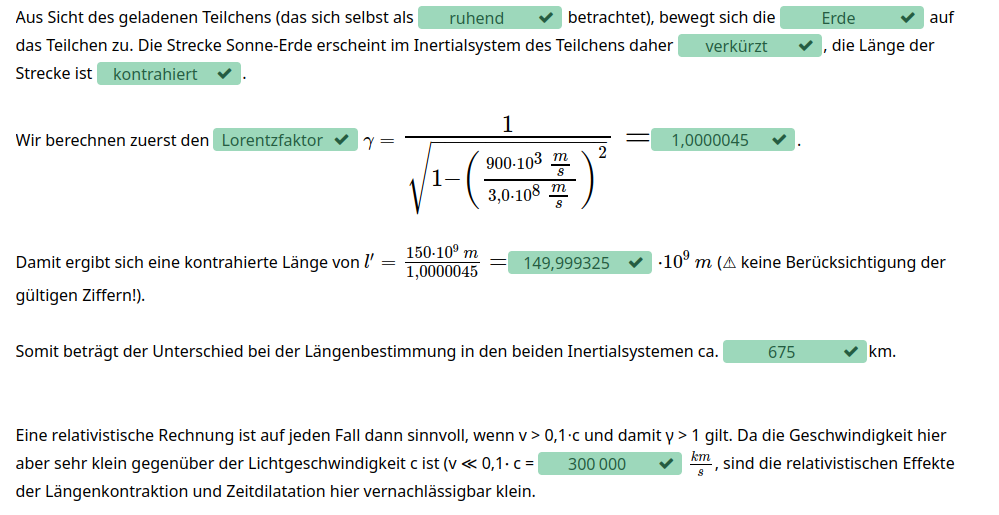
\includegraphics[scale=.5]{images/Lösung_Längenkontraktion.png}
	\end{figure}
\end{document}
